\documentclass[12pt]{beamer}

\usetheme{Air}
\usepackage{thumbpdf}
\usepackage{wasysym}
\usepackage{ucs}
\usepackage[utf8]{inputenc}
\usepackage{pgf,pgfarrows,pgfnodes,pgfautomata,pgfheaps,pgfshade}
\usepackage{verbatim}

\usepackage{tikz}
\usepackage{subfig}

\usepackage[absolute,overlay]{textpos}
\usepackage{graphicx}

\usetikzlibrary{fadings}
\usetikzlibrary{positioning}
\usetikzlibrary{arrows, matrix}

\pdfinfo
{
  /Title       (What limits fire, where and when?)
  /Creator     (CEH)
  /Author      (Douglas Kelley - douglas.i.kelley@gmail.com)
}

\title{What limits fire, where and when?}
\subtitle{Sensitivity of burnt area to different controls}
\author{Douglas Kelley, Ioannis Bistinas, Rhys Whitley, Toby Marthews, Chantelle Burton}
\date{December 15th 2016}

\titlegraphic{
\includegraphics[width=3.0cm]{logos/cehlogo945}\hspace*{1.6cm}~%
              
\includegraphics[width=1.5cm]{logos/ukesm-logo}\hspace*{1.6cm}~%
              
\includegraphics[width=3.0cm]{logos/nerc-long-logo-large}}

\begin{document}

\frame{\titlepage}
\pgfdeclareimage[width=1.0\paperwidth]{header-image}{header_images/fire}
%\section*{}
%\begin{frame}
%  \frametitle{Outline}
%  \tableofcontents[section=1,hidesubsections]
%\end{frame}

\AtBeginSection[]
{
  \frame<handout:0>
  {
    \frametitle{Outline}
    \tableofcontents[currentsection,hideallsubsections]
  }
}

\AtBeginSubsection[]
{
  \frame<handout:0>
  {
    \frametitle{Outline}
    \tableofcontents[sectionstyle=show/hide,subsectionstyle=show/shaded/hide]
  }
}

\newcommand<>{\highlighton}[1]{%
  \alt#2{\structure{#1}}{{#1}}
}

\newcommand{\icon}[1]{\pgfimage[height=1em]{#1}}



%%%%%%%%%%%%%%%%%%%%%%%%%%%%%%%%%%%%%%%%%
%%%%%%%%%% Content starts here %%%%%%%%%%
%%%%%%%%%%%%%%%%%%%%%%%%%%%%%%%%%%%%%%%%%

\section{Introduction}

\begin{frame}
    \frametitle{What controls fire}
    \framesubtitle{Is it people?}
    %Make clear we are talking about burnt area
\end{frame}

\section{Methods}

\begin{frame}
    \frametitle{Fire limitation framework}
    \framesubtitle{Spatial and Temporal controls on fire}

    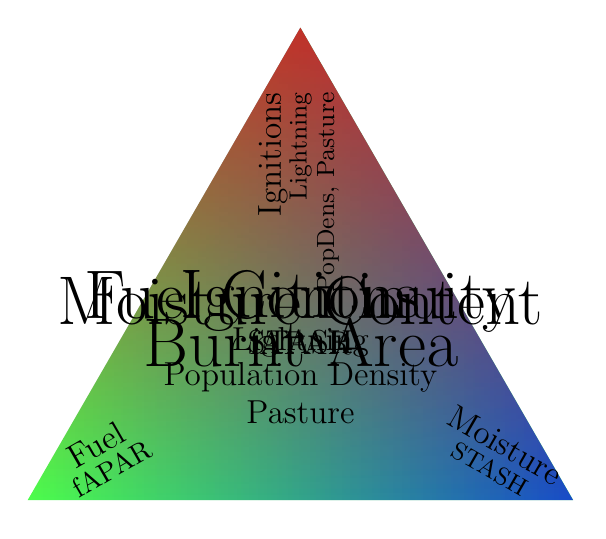
\begin{tikzpicture}
        \visible<2->{\fill[green, opacity = 0.7] (90:4) -- (210:4) -- (-30:4) -- cycle;}
        \visible<3->{\fill[blue,path fading=west, opacity = 0.7] (90:4) -- (210:4) -- (-30:4) -- cycle;}
        \visible<4->{\fill[red,path fading=south, opacity = 0.7] (90:4) -- (210:4) -- (-30:4) -- cycle;}

        \visible<2>{
            \node (note) at (0,1.5em) {\Huge Fuel Continuity};
            \node (note) at (0,0) { \large fAPAR};
        }

        \visible<3->{
            \node[rotate = 30] at (-2.6,-1.3) {\large Fuel};
            \node[rotate = 30] at (-2.4,-1.6) {fAPAR};
        }

        \visible<3>{
            \node (note) at (0,1.5em) {\Huge Moisture Content};
            \node (note) at (0,0) { \large STASH};
        }

        \visible<4->{
            \node[rotate = -30] at (2.6,-1.3) {\large Moisture};
            \node[rotate = -30] at (2.4,-1.6) {\small STASH};
        }

        \visible<4>{
            \node (note) at (0,1.5em) {\Huge Ignitions};
            \node (note) at (0,0) { \large Lightning};
            \node (note) at (0,-1.25em) { \large Population Density};
            \node (note) at (0,-2.5em) { \large Pasture};
        }

        \visible<5->{
            \node[anchor = east, rotate = 90] at (-1em,3.3) {\large Ignitions};
            \node[anchor = east, rotate = 90] at (0,3.3) {\small Lightning};
            \node[anchor = east, rotate = 90] at (1em,3.3) {\small PopDens, Pasture};
        }

        \visible<5>{
            \node (note) at (0,0) {\Huge Burnt Area};
        }

    \end{tikzpicture}


    \begin{textblock*}{5cm}(6.67cm,2cm)
        \visible<6->{
            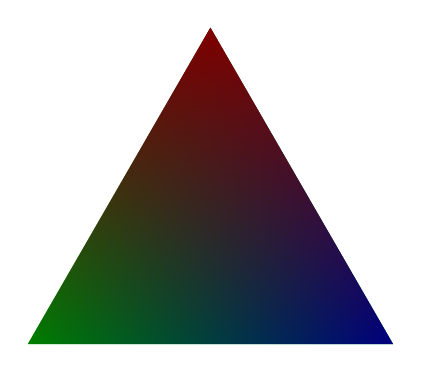
\begin{tikzpicture}[scale=0.67]
                \fill[green] (90:4) -- (210:4) -- (-30:4) -- cycle;
                \fill[blue,path fading=west] (90:4) -- (210:4) -- (-30:4) -- cycle;
                \fill[red,path fading=south] (90:4) -- (210:4) -- (-30:4) -- cycle;
                \fill[black, opacity = 0.5] (90:4) -- (210:4) -- (-30:4) -- cycle;
            \end{tikzpicture}
        }
    \end{textblock*}

    \begin{textblock*}{5cm}(10.1cm,2cm)
        \visible<7->{
            
\begin{tikzpicture}[scale=0.33]
                \fill[green] (90:4) -- (210:4) -- (-30:4) -- cycle;
                \fill[blue,path fading=west] (90:4) -- (210:4) -- (-30:4) -- cycle;
                \fill[red,path fading=south] (90:4) -- (210:4) -- (-30:4) -- cycle;
                \fill[black, opacity = 0.8] (90:4) -- (210:4) -- (-30:4) -- cycle;
            \end{tikzpicture}
        }
    \end{textblock*}

    \begin{textblock*}{4.5cm}(4.6cm,2.6cm)
        \visible<6->{
            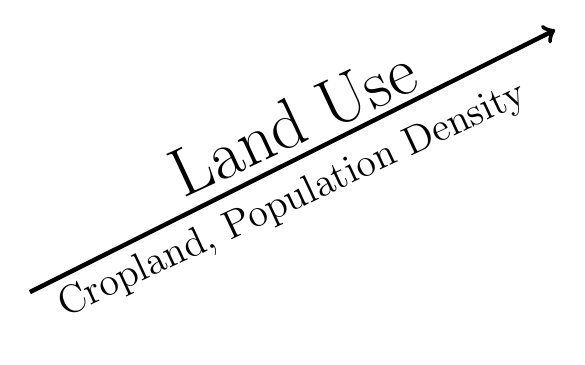
\begin{tikzpicture}
                \node[rotate = 25 ] (note) at (3.335, 2.165) {\Huge Land Use};
                    \node[rotate = 25 ] (note) at (3.335, 1.165) {\Large Cropland, Population Density};
                \draw[ultra thick, ->] (0, 0) -- (6.67, 3.33);
            \end{tikzpicture}
        }
    \end{textblock*}

    %Stuff to include:
    %   Monthly -> Inter annual and seasonal controls
\end{frame}

\section{Igntions}

\begin{frame}
    \frametitle{Igntions}
    \framesubtitle{Just Humans, Just natural, both combined}


\end{frame}

\begin{frame}
    \frametitle{Igntions}
    \framesubtitle{Igntion saturattion and manipulation}


\end{frame}

\section{Fragmentation}

\begin{frame}
    \frametitle{So Humans have no impact of fire?}
    \framesubtitle{Land use}
    %Start of with increase in burnt area from Igntions
    %Then add in land framgentation
\end{frame}

\begin{frame}
    \frametitle{Fire sensitivity}
\end{frame}

\section{Conclusion}

\begin{frame}
    \frametitle{Humans reduce burnt area}
    %Conclusions
    %Caviats
\end{frame}

\section{Example slides}

\begin{frame}
  \frametitle{Prerequisites \& Goals}
  \framesubtitle{Knowledge is a brick wall that you raise line by line forever}
  \begin{block}{LaTeX}
  \begin{itemize}
    \item Obviously some basic LaTeX knowledge is necessary
    \item Some more features will be provided here
  \end{itemize}
  \end{block}

  \begin{block}{Beamer}
  \begin{itemize}
    \item You'll learn them by looking at this presentation source
  \end{itemize}
  \end{block}

  \begin{block}{Goal}
  \begin{itemize}
    \item Learn how to make well structured slides
    \item Using a beautiful theme (congrats to the Oxygen team!)
    \item Take over the world
    \item Relax...
  \end{itemize}
  \end{block}
\end{frame}

\section{Basic structuring}
\begin{frame}
  \frametitle{Sections, Frames and Blocks}
  \framesubtitle{Put everything into boxes}

  The current section is "Basic structuring". And the current frame
  is what you have on the screen right now.

  \begin{block}{A beautiful block}
  A block has a title, and some content. You can put in a block
  almost everything you want that is provided by LaTeX. For example
  math works as usual:
    \begin{equation}
    \sum_{i=1}^n i = \frac{n \times (n+1)}{2}
    \end{equation}
  \end{block}

  Also works outside a block:
  \begin{equation}
  \sum_{i=1}^n i^2 = \frac{n \times (n+1) \times (2n+1)}{6}
  \end{equation}
\end{frame}

\begin{frame}
  \frametitle{Different type of blocks}
  \framesubtitle{Weeeee! Colors!!}
  \begin{block}{Standard block}
  \begin{itemize}
    \item A standard block, used for grouping
    \item Obviously can contain itemizes too...
    \begin{itemize}
      \item And nested itemizes...
      \item of course!
    \end{itemize}
  \end{itemize}
  \end{block}
  \begin{alertblock}{Alert block}
  WARNING: Something very important inside this block!
  \end{alertblock}
  \begin{example}
  Note that examples are displayed as a special block...
  \end{example}
\end{frame}

\section{Fancy features}
\begin{frame}
  \frametitle{Highlighting}
  \framesubtitle{Hey! Look here! here!}

  \begin{block}{A regular block}
  \begin{itemize}
    \item Normal text
    \item \highlighton{Highlighted text} to draw attention
    \item \alert{"Alert'ed" text} to spot very important information
    \item Alternatively you can
    \begin{itemize}
      \alert{\item "Alert" the item itself}
      \highlighton{\item Or "Highlight" it}
    \end{itemize}
  \end{itemize}
  \end{block}
  \begin{alertblock}{If it's very very important...}
  \alert{... you can "alert" in an "alertblock"}\\
  Ewww, nasty, heh?
  \end{alertblock}
\end{frame}

\newcommand{\putlink}[1]{%
   \pgfsetlinewidth{1.4pt}%
   \pgfsetendarrow{\pgfarrowtriangle{4pt}}%
   \pgfline{\pgfxy(1,1)}{\pgfxy(#1,1)}
}

\begin{frame}
  \frametitle{Overlay effects}
  \framesubtitle{Keep the suspense!}
  \begin{block}{Time bomb}
  \begin{enumerate}
    \item<2-> Two more to go
    \item<3-> One more to go
    \item<4-> Last chance...
    \item<5-> BOOM!
  \end{enumerate}
  \end{block}
  \begin{block}{"Animation"}<6->
    \begin{pgfpicture}{0cm}{0cm}{7cm}{2cm}
    \only<1-6>{
      \putlink{2}
    }
    \only<7>{
      \putlink{4}
    }
    \only<8>{
      \putlink{6}
    }
    \only<9>{
      \putlink{8}
    }
    \only<10>{
      \putlink{10}
    }
    \end{pgfpicture}
  \end{block}
\end{frame}

\section*{}
\frame{
  \vfill
  \centering
  \highlighton{
  \usebeamerfont*{frametitle}And now?

  \usebeamerfont*{framesubtitle}Enter the secret section
  }
  \vfill
}
\begin{frame}
  \frametitle{Contributing to this beamer style}
  \framesubtitle{We want you !}

  \begin{block}{Why?}
  \begin{itemize}
    \item Beamer is hot!
    \item This style deserves to be improved
  \end{itemize}
  \end{block}

  \begin{block}{How?}
  \begin{itemize}
    \item Grab it
    \item Improve its LaTeX code
    \item Use you artistics skills
    \item Document it
    \item Help other people to use it
    \item Use it...
  \end{itemize}
  \end{block}
\end{frame}

\begin{frame}
  \frametitle{Resources}
  \framesubtitle{If you want to improve this style}
  \begin{thebibliography}{10}

  \beamertemplatearticlebibitems

  \bibitem{beamer-homepage}
    LaTeX Beamer
    \newblock {\tt http://latex-beamer.sourceforge.net/}

  \bibitem{kdeslides}
    KDE Presentations
    \newblock {\tt http://www.kde.org/kdeslides/}

  \end{thebibliography}
\end{frame}

\frame{
  \vspace{2cm}
  {\huge Questions ?}

  \vspace{3cm}
  \begin{flushright}
    Konqi Konqueror

    \structure{\footnotesize{konqi@kde.org}}
  \end{flushright}
}

\end{document}
